Vorgängig zu dieser Arbeit wurden einige Teile davon in Vorleistung angegangen. Dies mit dem Ziel, sich in der eigentlichen Projektzeit voll und ganz auf die Elektronik und ggf. die Software zu konzentrieren. Diese Vorarbeiten beinhalten darum hauptsächlich Konstruktions- sowie Testaufbauten und werden im folgenden aufgezeigt. Dementsprechend sind alle in Kapitel \ref{vorarbeiten} behandelten Komponenten und Tests als bereits vorhanden, bzw. als Ausgangslage anzusehen.
\subsubsection{Konstruktion und Herstellung Prototyp}
Um das mechanische Verhalten einer Saite und die Herstellungsmethode mit Lasergeschnittenem MDF zu testen, wurde ein Prototyp konstruiert und hergestellt. Dieser bestand aus einem Resonanzkasten mit einer einzelnen Saite, Steg sowie einer Halterung für einen Rundmagneten. Abbildung \ref{pics:prototype} zeigt ein 3D-Rendering der Konstruktion, welche in Autodesk Fusion 360 konstruiert wurde. Anschliessend wurden MDF-Platten mit einem CO2-Lasercutter des Fablab Winterthur zugeschnitten und diese dann aufeinander geleimt. Somit konnten schon erste Tests durchgeführt werden.
\begin{figure}[H]
	\centering
	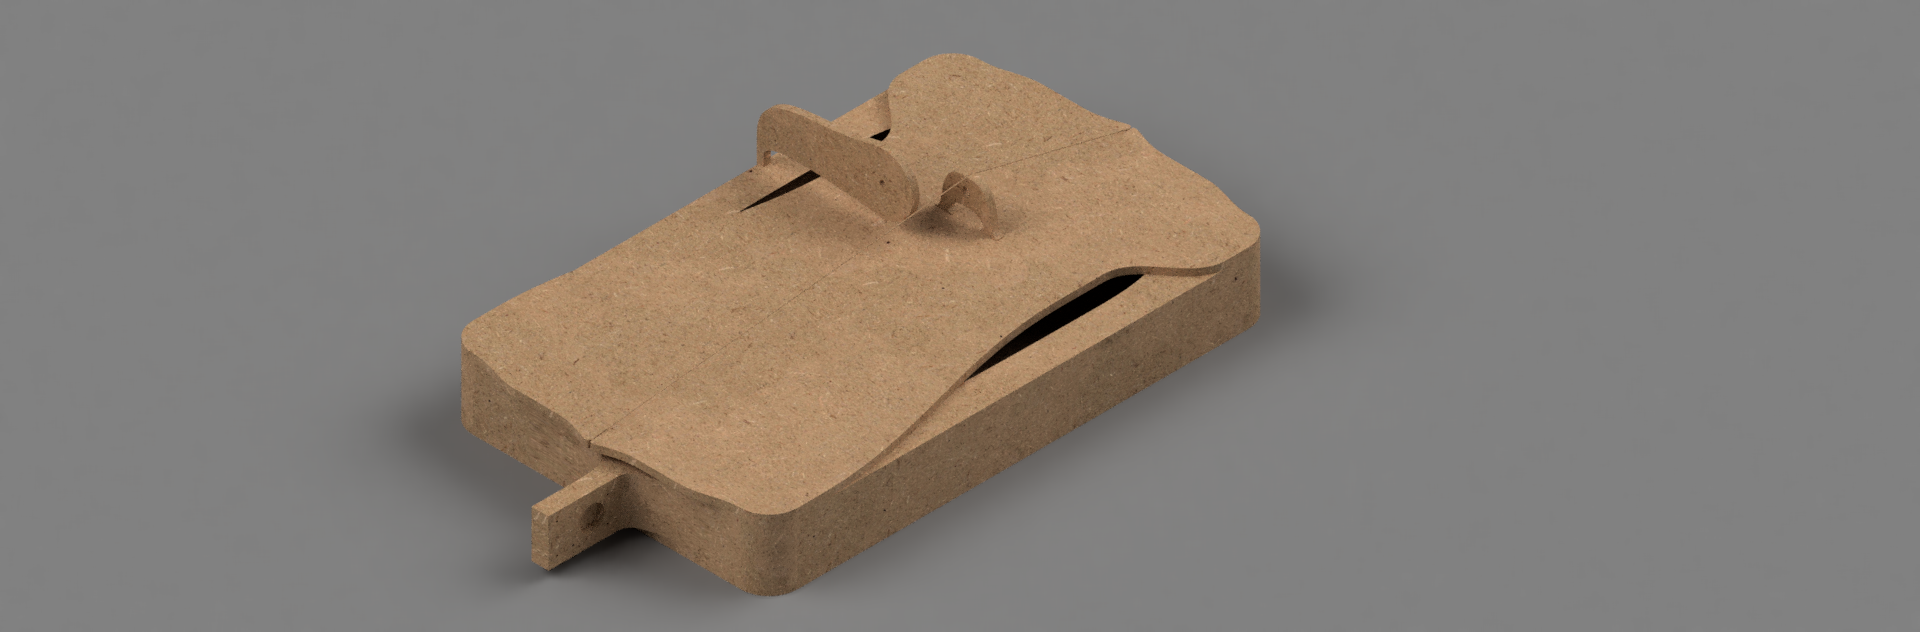
\includegraphics[width=\textwidth]{pictures/render_prototype.PNG}
	\caption{Rendering des Prototyps}
	\label{pics:prototype}
\end{figure}
\subsubsection{Schwingspulen}
Da noch unklar war, wie eine Saite am besten in Schwingung versetzt werden kann, wurden verschiedene Methoden getestet. Dabei wurden hauptsächlich drei Ansätze verfolgt:
\paragraph{Anregung mittels Schwingspule} Hierfür wurde Kupferdraht verschiedener Dicke um verschiedene Bobinen gewickelt und dann auf die Saite geleimt. Durch die Anwesenheit eines Magnetfeldes bewegt sich die Spule in Abhängigkeit des durchflossenen Stromes (Lorentzkaft). In Abbildung \ref{pics:all_voicecoils} sind einige Varianten aufgeführt. Getrieben wurde der Aufbau von einer analogen Endstufe. Hier zeigten sich schnell einige Herausforderungen: Oftmals war die Impedanz zu niedrig, oder die Hitzeentwicklung war zu stark. Ausserdem war ein grundsätzliches Problem, dass die Schwingspule sehr schnell zu rotieren begann, anstatt zu vibrieren und somit die Zuleitungen aufwickelte.
\begin{figure}[H]
	\centering
	\begin{subfigure}{0.7\textwidth}
		\centering
		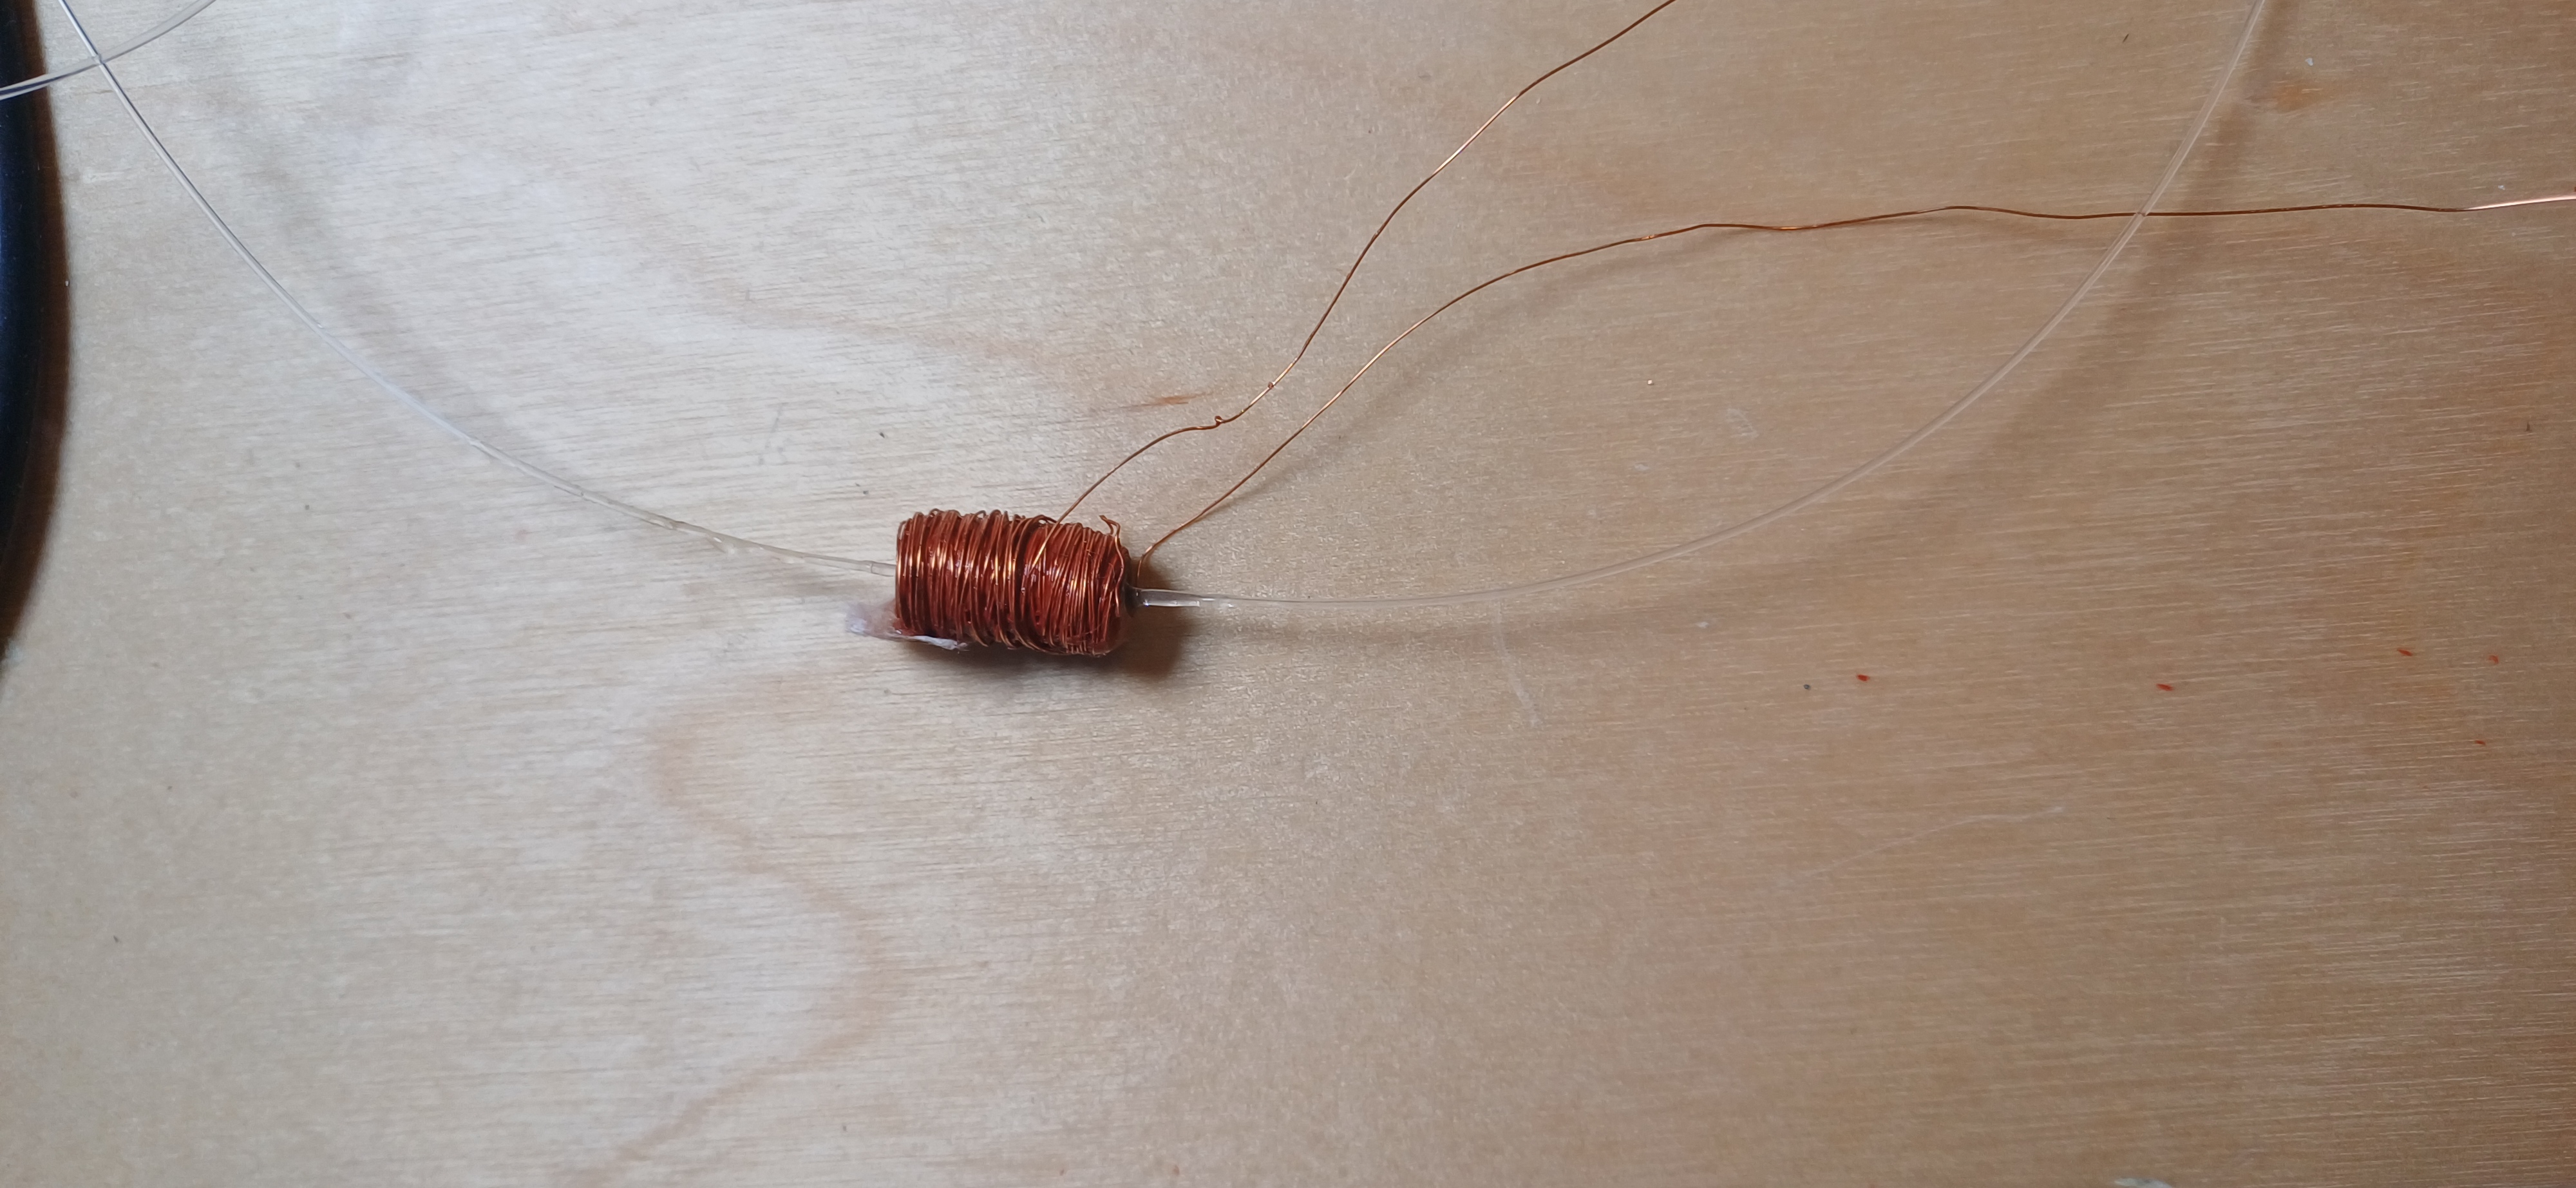
\includegraphics[width=\textwidth]{pictures/Schwingspule_lang.jpg}
		\caption{lange Schwingspule auf 5 Polymerbobinen}
		\label{pics:voicecoil_long}
		\vspace{4mm}
	\end{subfigure}\\
	\begin{subfigure}{0.7\textwidth}
		\centering
		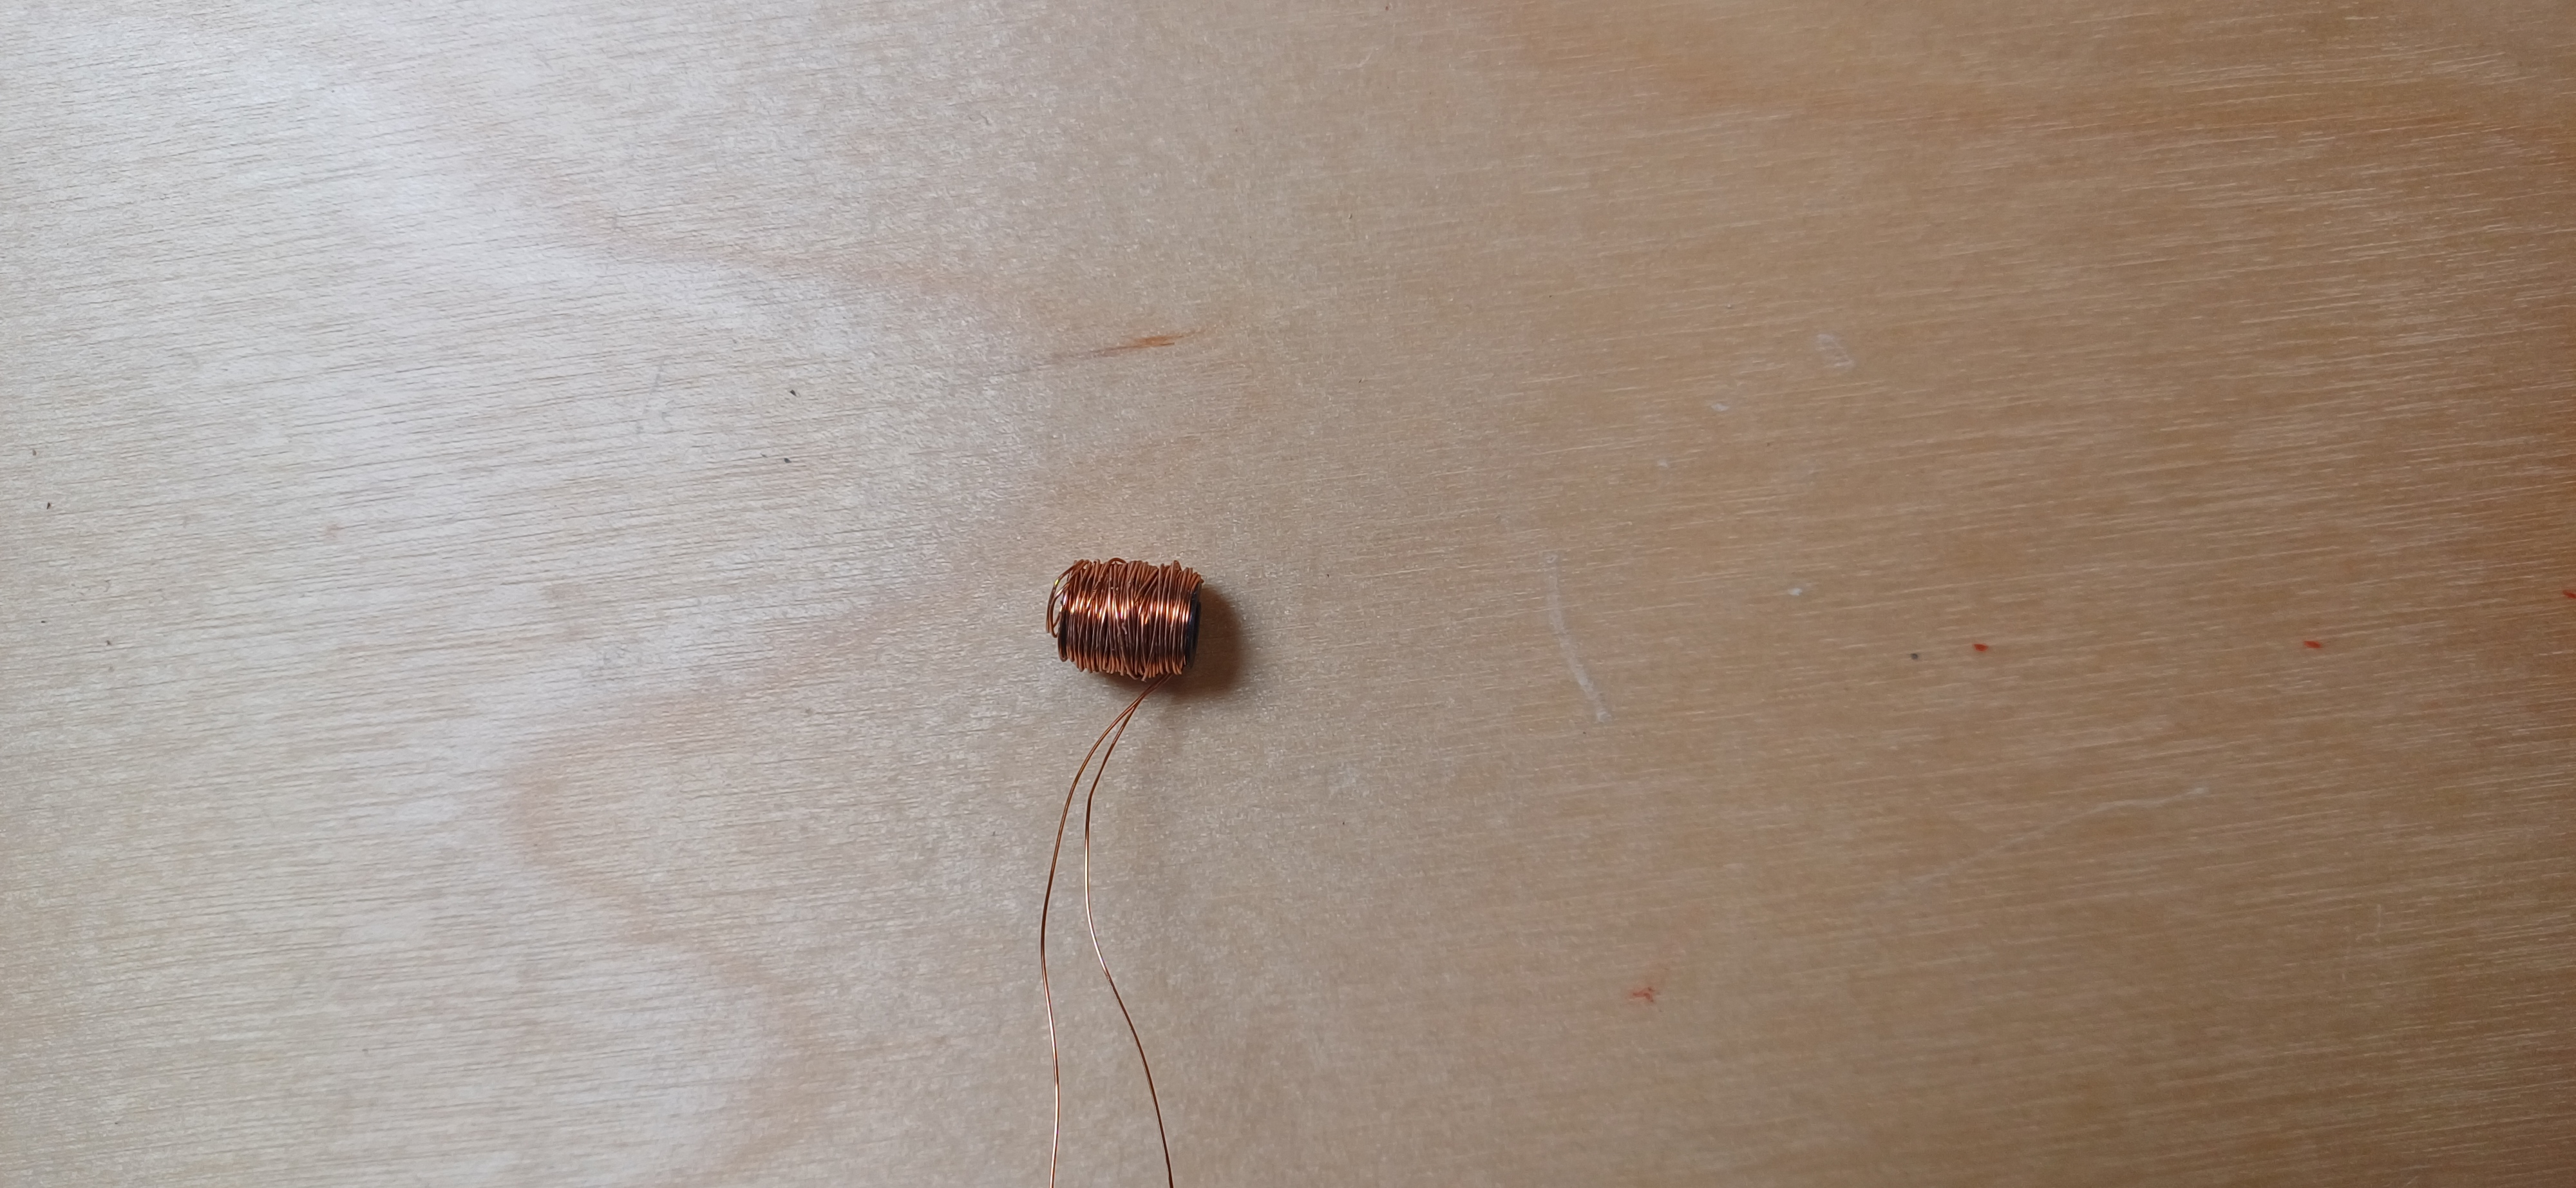
\includegraphics[width=\textwidth]{pictures/Schwingspule_kurz.jpg}
		\caption{kurze Schwingspule auf 3 Polymerbobinen}
		\label{pics:voicecoil_short}
		\vspace{4mm}
	\end{subfigure}\\
	\begin{subfigure}{0.7\textwidth}
		\centering
		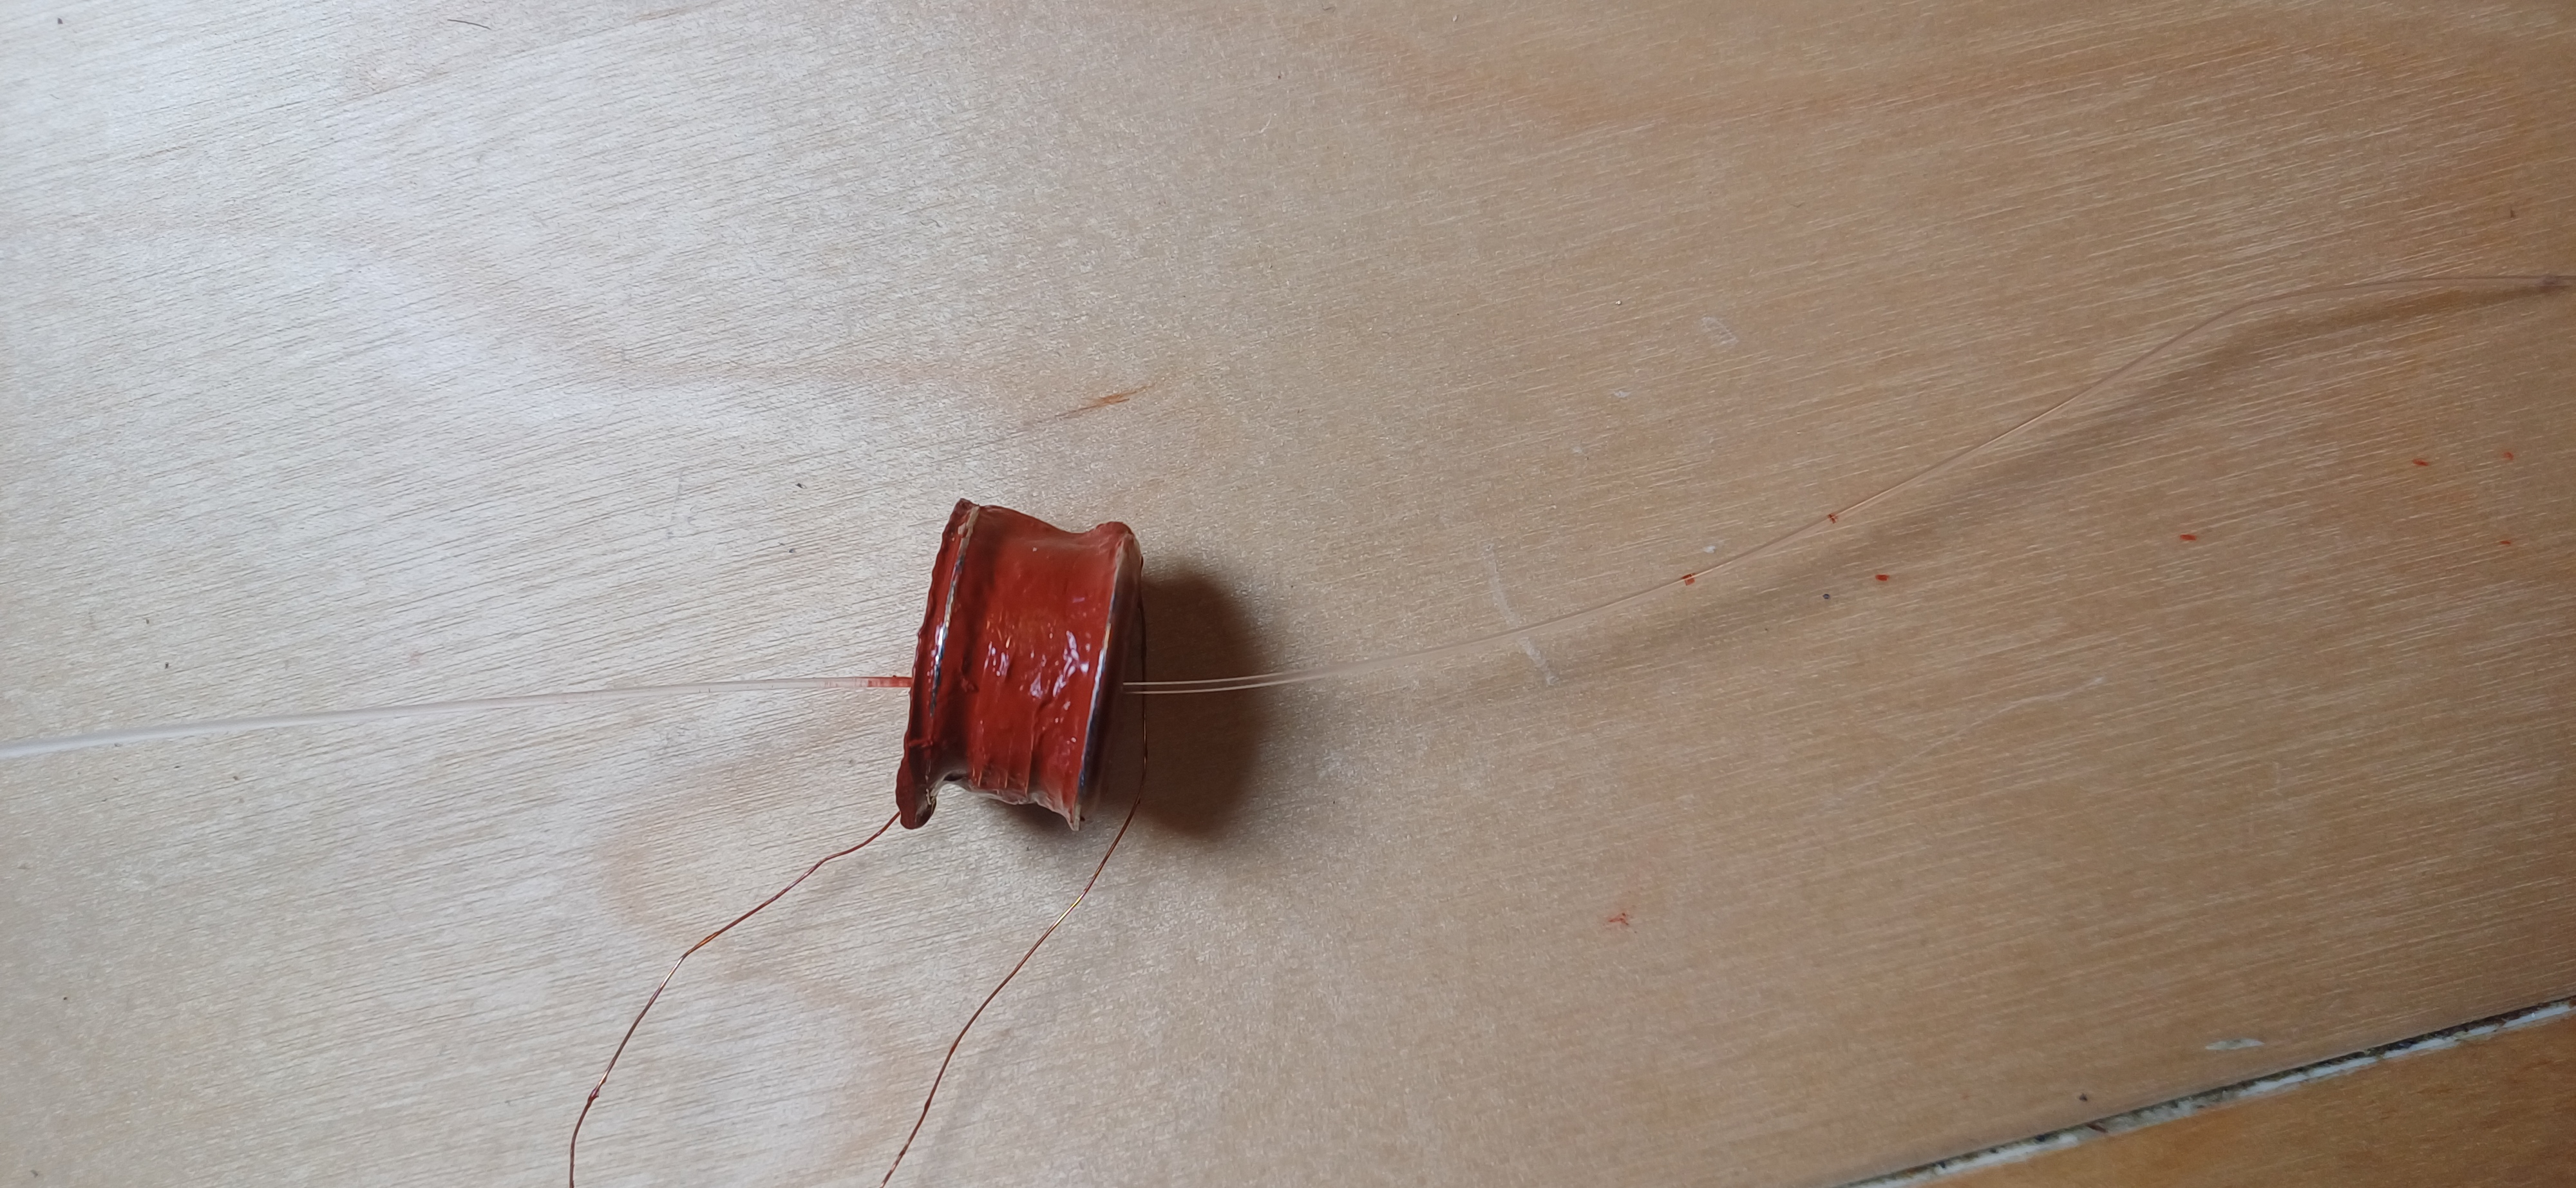
\includegraphics[width=\textwidth]{pictures/Schwingspule_eisenbobine.jpg}
		\caption{Schwingspule mit Eisenbobine, vergossen mit hitzebeständigem Kautschuk}
		\label{pics:voicecoil_iron}
		\vspace{4mm}
	\end{subfigure}
	\caption{verschiedene Schwingspulentypen}
	\label{pics:all_voicecoils}
\end{figure}
\noindent Des weiteren zeigte sich, dass ein einzelner Magnet neben einer Schwingspule die Spule nicht genügend mit einem Magnetfeld umschliesst. Die Bewegung blieb so sehr schwach. Weitaus besser funktionierte der Aufbau als zwei Magnete parallel montiert wurden und die Saite mit der Schwingspule dazwischen geführt wurde. So erzeugte die Schwingspule mit der Eisenbobine eine sehr starke Bewegung, konnte aber wegen des Rotationsproblems nicht verwendet werden.
\paragraph{Anregung mittels blanker Saite}
Eine sehr einfache Methode war es dann, den Signalstrom schlichtweg direkt durch die Saite zu leiten. Dabei wurde eine alte Instrumentensaite auf den Prototypen gespannt und Kontaktklemmen an den Enden angebracht. Zufälligerweise hatte die Saite eine Impedanz von ca. 3.2\Omega, wodurch sie direkt mit der Endstufe getrieben werden konnte.\\Dieser Aufbau hatte allerdings andere Limitationen: Ohne Wicklungen und Eisenkern blieb das erzeugte Magnetfeld der Saite sehr schwach. Zudem reagiert dieser Aufbau sehr stark auf die Resonanzfrequenz und deren harmonische Schwingungen, während andere Frequenzen kaum hörbar sind. {\color{red} VIDEO SWEEP} Somit liegt ein stark nicht-linearer Frequenzgang vor.
\begin{wrapfigure}{r}{0.5\textwidth}
	\vspace{10mm}
	\centering
	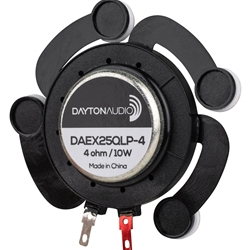
\includegraphics[scale=0.6]{pictures/exciter.jpg}
	\caption{DAEX25QLP-4 Exciter von Dayton Audio}
	\label{pics:exciter}
\end{wrapfigure}
\paragraph{Anregung mittels Exciter}
Ein weiterer Versuch bestand darin, einen Exciter, also sozusagen einen Lautsprecher ohne Membrane, auf den Prototypen zu platzieren. Somit wäre natürlich die Saite obsolet und der Begriff eines Saiteninstrument wohl nicht mehr zutreffend. Nichtsdestotrotz zeigte sich, dass dieser Aufbau um mehrere Zehnerpotenzen effektiver, also bisweilen auch ohrenbetäubend laut war. Auf der Innenseite montiert wäre das ganze Instrument schlichtweg eine unscheinbare Box welche auf Knopfdruck Klang abstrahlt\footnote{Das Prinzip existiert bereits als dekorative \textit{Flat Panel} oder \textit{Invisible Loudspeakers}}.
\subsubsection{Erkenntnisse}
\subsubsection{Konstruktion Korpus mit sechs Elementen}